\chapter{BFT Diversity Management}
\label{chap:lazarus_design}

 \note{We need to clarify that \system is proactive and \sieveq is reactive, they can be used together. E.g., when there is a problem the controller increases the risk}
\section{Introduction}


%This model only works if nodes fail independently, otherwise, once an attacker discovers a vulnerability in one node, it is most likely that the remaining nodes suffer from the same weakness. 

This paper presents \system, the first system that automatically changes the attack surface of a \gls{bft} system in a dependable way.
\system continuously collects security data from \gls{osint} feeds on the internet to build a knowledge base about the possible vulnerabilities, exploits, and patches related to the systems of interest.
This data is used to create clusters of similar vulnerabilities, which potentially can be affected by (variations of) the same exploit.
These clusters and other collected attributes are used to analyze the risk of the \gls{bft} system becoming compromised. % due to common vulnerabilities.
Once the risk increases, \system replaces the potentially vulnerable replica by another one, trying to maximize the failure independence. % of the replicated service.
Then, the replaced node is put on quarantine and updated with the available patches, to be re-used later.
These mechanisms were implemented to be fully automated, removing the human from the loop.

The current implementation of \system manages 17 \gls{os} versions, supporting the \gls{bft} replication of a set of representative applications.
The replicas run in \glspl{vm}, allowing provisioning mechanisms to configure them. 
We conducted two sets of experiments, one demonstrates that \system risk management can prevent a group of replicas from sharing vulnerabilities over time; the other, reveals the potential negative impact that virtualization and diversity can have on performance. However, we also show that if naive configurations are avoided, \gls{bft} applications in diverse configurations can actually perform close to our homogeneous bare metal setup.
%These results open avenues for many future works in the area. 

In summary, we make the following contributions: 

\begin{enumerate}

\item \system, a control plane that monitors \gls{osint} data and manages the \gls{bft} service replicas, selecting and reconfiguring the system to always run the ``most diverse'' set of replicas at any given time (Sections~\ref{sec:design} and~\ref{sec:implementation});

\item A method for assessing the risk of a group of replicas being compromised based on the security news feeds available on the internet. 
The method overcomes limitations from works that use NVD data for managing the replicas vulnerability independence (Section~\ref{sec:metric});

\item An evaluation of our risk management method based on real historical vulnerability data showing its effectiveness in keeping a group of replicas safe from common vulnerabilities (Section~\ref{sec:diversity});

\item An extensive evaluation of \system prototype using 17 \gls{os} versions, a \gls{bft} replication library, and some \gls{bft} applications (i.e., a \gls{kvs}, an application-level firewall/message queuing service, and a blockchain service) showing the costs of supporting diversity in \gls{bft} systems (Section~\ref{sec:overhead}).

\end{enumerate}



In a nutshell, as displayed in~Figure~\ref{fig:overview}, \system provides a distributed operating system for \gls{bft}-replicated services.
The system manages in its execution plane a set of nodes that can run \emph{unmodified replicas} (encapsulated in \glspl{vm} or containers). 
Each node must have a small \gls{ltu} that allows the activation and deactivation of replicas as demanded by the \system \emph{Controller}, in the control plane.
The controller decides which software should run at any given time by monitoring the existing vulnerabilities in the pool of replicas, aiming to minimize the risk of having several nodes being compromised by the same attack.

\begin{figure}[h]
\begin{center}
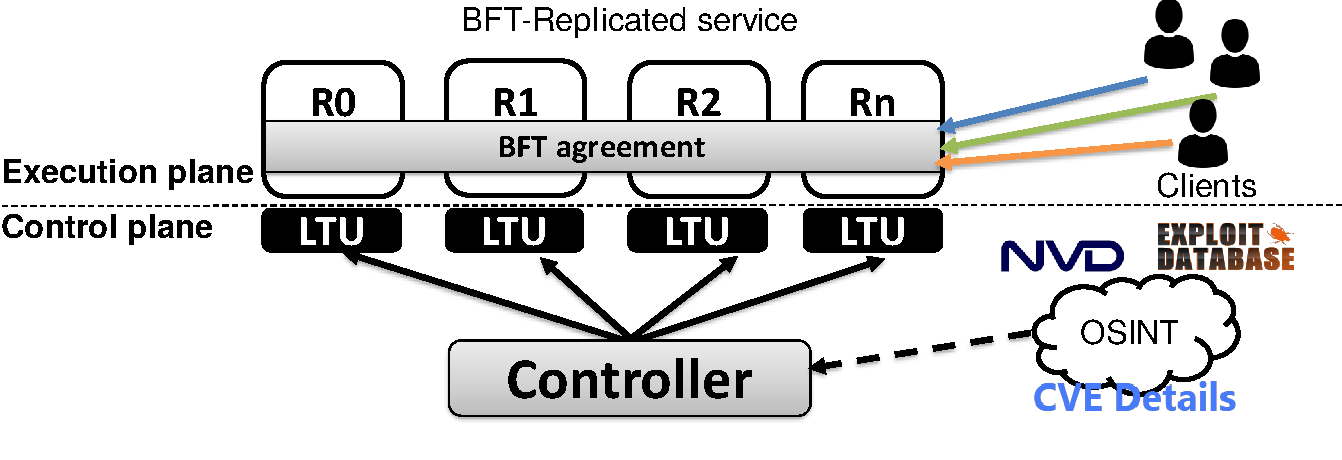
\includegraphics[width=0.7\columnwidth]{images/images/overview.pdf}
\vspace{-5mm}
\caption{\system overview.}
\label{fig:overview}
\end{center}
\end{figure}


\section{System Model}
\label{sec:systemmodel}

\system system model shares some similarity with previous works on the proactive recovery of \gls{bft} systems (e.g.,~\cite{Castro:2002,Platania:2014,Sousa:2010,Roeder:2010}).
More specifically, we consider a \emph{hybrid system model} composed of two planes with different properties and assumptions:

\begin{itemize}

\item \textbf{Execution Plane:} 
This plane is componsed of replica processes that can be subject to Byzantine failures.
Therefore, a Byzantine replica can try to mislead the other replicas or the clients.
These replicas communicate through an asynchronous network that can delay, drop or modify messages, just like most \gls{bft} system models~\cite{Castro:1999,Kotla:2010,Bessani:2014,Aublin:2015}.
This plane hosts $n$ replicas from which at most $f$ can be compromised at any given moment.
In this paper, we consider the typical scenario in which $n=3f+1$~\cite{Castro:2002,Kotla:2010,Aublin:2015}.  

\item \textbf{Control Plane:}  
For simplicity, we will address this component as a logical-centralized controller, which requires stronger assumptions. 
However, in Chapter~\ref{} we introduce \controller which requires weaker assumptions like the Execution Plane.

In this plane, we assume that each component can only fail by crashing. 
Each \emph{node} hosting processes contains a \gls{ltu}, and there is a logically-centralized controller to reconfigure the system, just like what has been used in several previous works on proactive recovery (e.g.,~\cite{Roeder:2010,Platania:2014,Sousa:2010}).
The failures of such components do not compromise the liveness and safety of the service as long as the control plane is recovered before $f$ replicas fail.


\end{itemize}

Besides the execution and control planes, we assume the existence of two types of external components: (1) clients of the replicated service, which can be subject to Byzantine failures; (2) \gls{osint} sources (e.g., \gls{nvd}, ExploitDB) that can not be subverted and controlled by the adversary.
In practice, this assumption lead us consider only well-established and authenticated data sources.
Dealing with untrusted sources is an active area of research in the threat intelligence community (e.g.,~\cite{Sabottke:2015,Liu:2015}), which we consider out of scope for this paper.


\section{Execution Plane}
\label{sec:executionplane}

The Execution Plane can accomodate any replicated system that already levareges on the existence of a controller node (e.g.,~\cite{Sousa:2010,Roeder:2010,Platania:2014,Garcia:2016}) or any \gls{bft} system that would benefit from the \system assistence (e.g.,~\cite{Sousa:2018}). 


\section{Control Plane}
\label{sec:controlplane}

\system is the first control plane that automatically changes the attack surface of a \gls{bft} system in a dependable way.
\system continuously collects security data from \gls{osint} feeds on the internet to build a knowledge base about the possible vulnerabilities, exploits, and patches related to the systems of interest.
This data is used to create clusters of similar vulnerabilities, which potentially can be affected by (variations of) the same exploit.
These clusters and other collected attributes are used to analyze the risk of the \gls{bft} system becoming compromised. % due to common vulnerabilities.
Once the risk increases, \system replaces the potentially vulnerable replica by another one, trying to maximize the failure independence. % of the replicated service.
Then, the replaced node is put on quarantine and updated with the available patches, to be re-used later.
These mechanisms were implemented to be fully automated, removing the human from the loop.

The current implementation of \system manages 17 \gls{os} versions, supporting the \gls{bft} replication of a set of representative applications.
The replicas run in \glspl{vm}, allowing provisioning mechanisms to configure them. 
We conducted two sets of experiments, one demonstrates that \system risk management can prevent a group of replicas from sharing vulnerabilities over time; the other, reveals the potential negative impact that virtualization and diversity can have on performance. 
However, we also show that if naive configurations are avoided, \gls{bft} applications in diverse configurations can actually perform close to our homogeneous bare metal setup.

\section{Diversity of Replicas}
\label{sec:diversityofreplicas}
\note{citar survey \cite{Baudry:2015}}
%BFT-replicated services running on \system are composed by $n$ replicas.
For our purposes, each \replica is composed of a stack of software, including an OS (kernel plus other software contained in an \gls{os} distribution), execution support (e.g., \gls{jvm}, \gls{dbms}), a \gls{bft} library, and the service that is provided by the system.
%(see Figure~\ref{fig:arch1}).
The set of $n$ replicas is called a \configuration.

It is possible to improve the \replicas fault independence by resorting to different \gls{ots} components in the software stack~\cite{Deswarte:1998}. 
For example, it has been shown that using distinct \glspl{os}~\cite{Garcia:2014}, filesystems~\cite{Rodrigues:2001,Bairavasundaram:2009}, and databases~\cite{Gashi:2007}, can yield important benefits in terms of fault independence. In addition, automatic techniques could enhance diversity, like randomization/obfuscation of \glspl{os}~\cite{Roeder:2010} and applications~\cite{King:2016}.

Although \system can exploit automatic techniques, in this paper we center our attention on diverse \gls{ots} components. 
In particular, \system monitors the disclosed vulnerabilities of all elements of the software stacks of the replicas to assess which of them may contain common vulnerabilities.  

However, in the experimental evaluation, we focus on the diversity of OSes (not only the kernel, but the whole product) for three fundamental reasons: (1) by far, most of the replica’s code is the \gls{os}; (2) such size and importance, make \glspl{os} a valuable target, with new vulnerabilities and exploits being discovered every day; and (3) there are many options of OSes that can be used.
The two last factors are particularly important to enrich the validity of our analysis.

Moreover, we do not explicitly consider the diversity of the \gls{bft} library (i.e., the protocol implementation) or the service code implemented on top of it.
Four facts justify this decision: (1) N-version programming is too costly for this~\cite{Avizienis:1977}; (2) there have been some works showing that such protocol implementations can be generated from formally verified specifications~\cite{Hawblitzel:2015,Rahli:2018}; (3) the relatively small size of such components (e.g., a key-value store on top of BFT-SMaRt has less than 15k lines of code~\cite{Bessani:2014}) make them relatively simple to test and assess with some confidence~\cite{Martins:2013,Lee:2014};  and (4) there are no reported vulnerabilities about these system to support our study.
Notice that, although we do not explicitly consider the diversity of \gls{bft} libraries, nothing prevents \system from monitoring them (when several alternatives become available). 
Additionally, as a pragmatic approach, we could employ automatic diversity techniques in this layer~\cite{Platania:2014,Roeder:2010}.




\section{Diversity-aware Reconfigurations}
\label{sec:metric}

The core of \system is the vulnerability evaluation method used to assess the risk of having replicas with shared vulnerabilities.
This section details this method.

\subsection{Finding Common Vulnerabilities}

%\gls{nist}'s \gls{nvd}~\cite{nvd} is the authoritative data source for disclosure of vulnerabilities and associated information~\cite{Massacci:2010}. 
%\gls{nvd} aggregates vulnerability reports from more than 70 security companies, advisory groups, and organizations, thus being the most extensive vulnerability database on the web. 
%All data is made available as \gls{xml} data feeds, containing the reported vulnerabilities on a given period. 
%Each \gls{nvd} vulnerability receives a unique identifier and a short description provided by the \gls{cve}~\cite{cveterm}. 
%The \gls{cpe}~\cite{cpe} provides the list of products affected by the vulnerability and the date of the vulnerability publication.
%The \gls{cvss}~\cite{cvss} calculates the vulnerability severity considering several attributes, such as the attack vector, privileges required, exploitability score, and the security properties compromised by the vulnerability (i.e., integrity, confidentiality, or availability).
WE USE THE NVD (as described in Chapter~\ref{chap:datasource}


Previous studies on diversity solely count the number of shared vulnerabilities among different \glspl{os}, assuming that less common vulnerabilities implies a smaller probability of compromising $f+1$ OSes~\cite{Garcia:2014}. 
Although this intuition may seem acceptable, in practice it underestimates the number of shared vulnerabilities due to imprecisions in the data sources. 
For example, Table~\ref{tab:missing_products} shows three vulnerabilities, affecting three different \glspl{os} at distinct dates.
At first glance, one may consider that these \glspl{os} do not share vulnerabilities.
However, a careful inspection of the descriptions shows that they are very similar.
Moreover, we checked this resemblance by searching for additional information on security web sites, and we found out that CVE-2016-4428, for example, also affects Solaris.\footnote{\url{https://www.oracle.com/technetwork/topics/security/bulletinjul2016-3090568.html}}

\begin{table}[!t]
\begin{center}
{\scriptsize
\begin{tabular}{| p{2.3cm} | p{10cm} | }\hline
\textbf{CVE (affected OS)} & \textbf{Description} \\\hline\hline
CVE-2014-0157 (Opensuse 13) & \scriptsize \gls{xss} vulnerability in the Horizon Orchestration dashboard in OpenStack Dashboard (aka Horizon) 2013.2 before 2013.2.4 and icehouse before icehouse-rc2 allows remote attackers to inject arbitrary web script or HTML via the description field of a Heat template. \\ \hline
CVE-2015-3988 (Solaris 11.2) & \scriptsize Multiple \gls{xss} vulnerabilities in OpenStack Dashboard (Horizon) 2015.1.0 allow remote authenticated users to inject arbitrary web script or HTML via the metadata to a (1) Glance image, (2) Nova flavor or (3) Host Aggregate. \\ \hline
CVE-2016-4428 (Debian 8.0) & \scriptsize \gls{xss} vulnerability in OpenStack Dashboard (Horizon) 8.0.1 and earlier and 9.0.0 through 9.0.1 allows remote authenticated users to inject arbitrary web script or HTML by injecting an AngularJS template in a dashboard form. \\ \hline
\end{tabular}
}
\caption{Similar vulnerabilities affecting different OSes.}
\label{tab:missing_products}
\end{center}
\end{table}

Even with these imperfections, \gls{nvd} is still the best data source for vulnerabilities.
Therefore, we exploit its curated data feeds for obtaining the unstructured information present in the vulnerability text descriptions and use this information to find similar weaknesses.
A usual way to find similarity in unstructured data is to use clustering algorithms~\cite{Jain:2010}.
Clustering is the process of aggregating related elements into groups, named clusters, and is one of the most popular unsupervised machine learning techniques. 
We apply this technique to build clusters of similar vulnerabilities (see Section~\ref{sec:details} for details), even if the data feed reports that they affect different products.
For example, the vulnerabilities in Table~\ref{tab:missing_products} will be placed in the same cluster as there is some resemblance among the descriptions, and they can potentially be activated by (variations of) the same exploit.

It is worth to remark that by using clusters to find similar vulnerabilities, we conservatively increase the chances of capturing shared weaknesses contributing to the score of a pair of replicas.

\subsection{Measuring risk}
\label{sec:measurerisk}

As discussed before, each vulnerability in \gls{nvd} has an associated \gls{cvss} severity score. 
Therefore, a straw man solution for measuring risk would be to sum the \gls{cvss} scores of all common vulnerabilities in the software stack of two replicas to get an estimate of how dangerous are their shared weaknesses.
However, \gls{cvss} has some limitations that make it unsuitable for managing the risk of replicated systems:
(1) In practice, it has been shown that there is no correlation between the \gls{cvss} exploitability score and the existence of real exploits for the vulnerability~\cite{Bozorgi:2010}; 
(2) \gls{cvss} does not provide information about vulnerabilities exploiting and patching times; 
(3) \gls{cvss} does not account for the vulnerability age, which means that severity remains the same over the years~\cite{Frei:2006,Melo:2013}; 
and (4) some studies show that \gls{cvss} may overestimate  severity~\cite{Sabottke:2015}, as for example larger scores do not correspond to higher prices in the vulnerabilities' black markets~\cite{Allodi:2014}.

Given these limitations, we derive a novel, more refined, metric to measure the risk of a \gls{bft} system being affected by common vulnerabilities.
In our particular context, we are mostly interested in capturing information that relates to the window of exposure that vulnerabilities have, mainly when they are correlated among \replicas.
Therefore, we developed a risk metric that aims to overpass the identified limitations. 
We solved (1) and (2) by using additional \gls{osint} sources that provide information about the exploit and patch dates. 
Since NVD does not provide this information, we collect more data from other \gls{osint} sources like Exploit-DB~\cite{edb} for exploits, patching information from CVE-details~\cite{cvedetails}, and additional vendor websites, such as Ubuntu Security Notices~\cite{ubuntu}, Debian Security Tracker~\cite{debian}, and Microsoft Security Advisories and Bulletins~\cite{microsoft} (which also give additional product versions affected by the vulnerability).
We solve (3) using the vulnerability published date to calculate its age.
Finally, we only use the \gls{cvss} attributes that concern to integrity and availability, the properties traditionally related with \gls{bft} replication (4).


\begin{table}[h]
\begin{center}
{\small
\begin{tabular}{ c }\hline
\vbox{
\begin{equation}
\mathit{\systemformula(sc)}=\sum_{i=1}^{n-1} \sum_{j=i+1}^{n} \pairformula(rc_i,rc_j) \label{eq:3}
\end{equation}
}\\ \hline
\vbox{
\begin{equation}
\mathit{\pairformula(rc_i,rc_j)}=\sum_{v_k \in \mathcal{V}_{i,j}} \mathit{\vulnerabilityformula(v_k)} \label{eq:2}
\end{equation}
}\\ \hline
\vbox{
\begin{equation}
\mathit{\vulnerabilityformula(v_k)}= (A+I+\mathit{exp(v_k)}) \times \mathit{tdist(v_k)} \label{eq:1}
\end{equation}
\begin{equation}

\mathit{exp(v_k)}= \begin{cases}
		\mathit{max(\mathit{DP}-\mathit{DE},0)}+1 	& \text{$v_k$ exploited, patched}\\
  		\mathit{DE} 		& \text{$v_k$ exploited, not patched}\\
		0 		& \text{otherwise}
\end{cases} \label{eq:exposed}
\end{equation}
}\\ \hline

\end{tabular}
}
\label{tab:equations}
\end{center}
\end{table}

Our metric considers all this information to measure the risk of a set of $n$ replicas having active shared vulnerabilities.
More specifically, it works as an indicator of how fault-independent is a \configuration.
Equation~\ref{eq:3} shows the risk of a \configuration as the sum of the different \replica pairs' score.
This score is calculated based on the set of vulnerabilities $\mathcal{V}_{i,j}$ that affects both $r_i$ and $r_j$ or that are present in a cluster containing vulnerabilities affecting both \replicas (Equation~\ref{eq:2}).
Finally, we calculate the score of each vulnerability in $\mathcal{V}_{i,j}$ (Equation~\ref{eq:1}). 
We assign a \emph{dynamic score} to each vulnerability, considering the referred attributes:
\emph{(i)} we take two \gls{cvss} attributes to capture the extent to which a vulnerability $v_k$ affects availability ($A$) and integrity ($I$);
\emph{(ii)} we account for the number of days the vulnerability was exposed with $\mathit{exp}$, i.e., there was an exploit and no patch available.
This is calculated considering the number of days to patch ($DP$) and to exploit ($DE$) $v_k$ (Equation~\ref{eq:exposed}); 
\emph{(iii)} and we use an amortization function to reflect the fact that older vulnerabilities have are less likely to harm the system ($\mathit{tdist(v_k)} \in [0,1]$).


\subsection{Selecting Configurations}
\label{sec:configurations}


We use the risk metric to choose the \replicas that should be included in the \configuration. 
This is done by periodically evaluating the risk of the current \configuration. 
If the risk exceeds a pre-defined threshold, a mechanism is triggered to replace replicas and reduce the overall risk.
First, it decides which \replica (\r) should be removed and put in a quarantine set (\QS). 
Then, it selects (one of) the best candidate(s) replicas from all the available candidates (\RS) to make the substitution.
When the replacement takes place, the resulting \configuration (\ES) has lower risk than the previous one.
Additionally, we ensure that removed \replicas can sometime later re-enter the system, and the ones that are in the system, despite their overall score, are eventually replaced.
Therefore, each replica \r in \ES has an \emph{age} value that is incremented. 
On the contrary, each removed replica \r in \QS, has a \emph{healing} value that is decremented.


This procedure is detailed in Algorithm \ref{alg:algorithm2}.
The \emph{Monitor} function is called on each monitoring round (e.g., on every hour).
Consider a \ES that is already running with risk$=\alpha$.
First, the algorithm increments the \emph{age} of each \r in \ES (lines 6-7).
Then, it verifies if the risk of \ES (Equation~\ref{eq:3}) does not exceed the predefined $\mathit{threshold}$ (line 8).
In the affirmative case, a \replica replacement is started.
First, some local variables are initialized (lines 9-10).
Second, it randomly gets pairs $\langle i,j \rangle$ from \ES (line 11) and saves some of them that augment the risk in \MAX (Equation~\ref{eq:2}) (lines 12-14). 
Third, the algorithm picks the older replica (i.e., the one that is in \ES for more time) of all selected pairs (lines 15-18). 
This replica is removed from \ES (line 19) and added to \QS (line 21).
The \emph{healing} value is initialized with a value, different for each \replica, based on historical data about the time it takes for a patch to be published for this software (line 20). 
The algorithm calls a function that selects a new replica to join \ES (line 22). Finally, it decrements the \emph{healing} of each \r in \QS (line 24). When such value reaches zero, \r is removed from \QS and added to \RS (lines 25-28).

Function \emph{Find\_new\_config()} (line 22) solves the following optimization problem:

\vbox{
\begin{small}
\begin{equation*}
\begin{array}{ll@{}ll}
\text{\underline{min} } & \emph{risk}(\ES \cup \{r\}) 	 	\\
\text{\underline{subject to}}	&	 r \in \RS 			\\ 
\end{array}
\end{equation*}
\end{small}
}

\noindent
where \ES is the set of $n-1$ replicas that will stay in the system and $r$ is the new replica (which we have to find) among the ones in \RS.
The twist in our case is that we avoid deterministic solutions to increase the difficulty of an adversary guessing the next configurations.
Therefore, we developed a simple heuristic that finds the $k$ best replicas in \RS (e.g., $k=3$) and randomly picks one of them to be added to \ES.
The heuristic is quite simple: we just calculate the risk of a configuration with each candidate replica from \RS, and choose one of the $k$ replicas that induce lower risk. 

%The minimization problem presented is similar to a problem of solving the minimal cost of a $n$-clique for complete graphs. 
%However, as we mentioned before, we want to create unpredictability on the results.
%Therefore, we introduce randomness on the selection, meaning that the solution is minimal but not always the minimum.
%The minimization function (line 22) is a heuristic to select the valid candidates to reconfigure the \ES with a smaller $\alpha$ than before. 
%The selection of \r must have some degree of unpredictability to increase the difficulty of guessing future configurations.
%To meet this goal, we add randomness when picking \replicas while restricting the number of candidate elements to the ones that minimize the risk. 
%It starts iterating over the \RS and uses the Equation~\ref{eq:3} to calculate the risk of such configuration (line 30).
%If the risk is under a predefined $threshold$, the candidate \r is initialized (line 32), removed from the \RS (line 33) and added to a set with the admissible candidates (\PS) (line 34).
%Then, a random \r is picked from \PS and added to \ES (line 35) which is then returned (line 36).

Although better heuristics can be developed, this brute-force method works in \system because we do not expect \RS (our solution space) to be large.
In addition, this function is only called if the risk exceeds the threshold. 

{\centering
\begin{minipage}{.7\linewidth}
  \begin{algorithm}[H]
\caption{Replica Set Reconfiguration}\label{alg:algorithm2}
{\footnotesize
%\N: number of replicas\;
%\K: number of replicas to remove\;
\ES: set replicas in the \configuration \;
\RS: set with the available replicas (not in use)\;
%\CS: set of candidate replicas\;
%\RM: set of removable replicas\;
\MAX: set of candidate replicas to remove\;
\QS: set of quarantine replicas\;
%\PS: set of valid replicas\;

\BlankLine
\Fn{Monitor ()}{
	\ForEach{r in \ES}{
		\Inc{r.age};
	}
	\If{\Risk{\ES} $>$ threshold}{
		$maxScore$, $maxAge$ $\leftarrow$ 0\;
		\toRemove $\leftarrow$ $\perp$\;
%		\While{\Size{\toRemove} $<$ \K}{
			\ForEach{$\langle i,j \rangle$ in \ES}{
				\If{\Common{i,j} $\geq$ maxScore}{	
					\MAX $\leftarrow$ \MAX $\cup$ $\{\langle i,j \rangle\}$\;
					$maxScore$ $\leftarrow$ \Common{i,j}\;
				} 
			}
				\ForEach{$\langle i,j \rangle$ in \MAX}{
					\If{\Older{i,j} $\geq$ maxAge}{	
						\toRemove $\leftarrow$ \Older{i,j}\;
						$maxAge$ $\leftarrow$ \toRemove.age\;	
					} 
			}		
			 \ES $\leftarrow$ \ES $\setminus$ $\{$ \toRemove$\}$\;	
             $\toRemove$.healing $\leftarrow$ \healing{\toRemove}\;
			 \QS $\leftarrow$ \QS $\cup$ $\{$ \toRemove$\}$\;
%		}
		 \ES $\leftarrow$ $\mathit{Find\_new\_config(\RS, \ES)}$\;
	}
	\ForEach{r in \QS}{
		\Dec{r.healing}\;
		\If{r.healing $=$ 0}{		
			\QS $\leftarrow$ \QS $\setminus$ $\{r\}$\;		
			$r.age$ $\leftarrow$ 0\;
            \RS $\leftarrow$ \RS $\cup$ $\{r\}$\;
		}
	}
}
%\Fn{Minimize (\RS, \ES)}{
%%	\If{\Size{\ES} is $\emptyset$}{
%%		\CS $\leftarrow$ $\emptyset$\;
%%		\CS $\leftarrow$ \Rand{\RS}\; 
%%	}
%%	\While{\Size{\CS} $\leq \N$}{
%		\PS $\leftarrow$ $\{\}$\;
%		\ForEach{r in \RS}{
%			\If{\Risk{\ES $\cup$ r} $<$ threshold}{
%				r.age $ \leftarrow$ 0\;
%				\RS $\leftarrow$ \RS $\setminus$ $\{r\}$\;		
%				\PS $ \leftarrow$ \PS $\cup$ $\{r\}$\;
%			}
%		}
%		\ES $\leftarrow$ \ES $\cup$ $\{\Rand{\PS}\}$\;
%%	}
%\Return	\ES\;
%}
%\end{multicols}
}
\end{algorithm}

\end{minipage}
\par
}


\section{Evaluation of Replica Set Risk}
\label{sec:diversity}

This section evaluates how \system performs on the selection of dependable \replica configurations.
As discussed in Section~\ref{sec:replica}, we focus our experimental evaluation solely on the OS diversity.
% These play a crucial role in any IT system, and most of the \replica's code is the OS. 
% Thus, they present a high potential to become the most vulnerable part of a \replica.
% Hence, in the following experiments, we explore OS diversity among the replicas. 

In these experiments, we emulate live executions of the system by dividing the collected data into two periods:
(i) a \emph{learning phase} covering all vulnerability data between \emph{2010-1-1} and \emph{2017-9-29}, which is used to setup the \risk's algorithm; and (ii) an \emph{execution phase} composed of the period between \emph{2017-10-1} and \emph{2018-3-30}.
This last period is divided into three intervals of two months (OUT-NOV, DEC-JAN, and FEB-MAR), allowing for three independent tests.
%JAN-FEB, MAR-APR, and MAY-JUN
The goal is to create a knowledge base in the \emph{learning phase} that is used to assess \system choices during each interval of the \emph{execution phase}. 
A run starts on the first day of an interval and then progresses through each day of the interval until the end. Every day, we check if the currently executing replica set could be compromised by an attack exploring the vulnerabilities released on that day. 
We take the most pessimist approach, which is to say that we consider the system to be broken if a vulnerability comes out that affects at least two OSes that would be executing at that time.

Three additional strategies, inspired by previous works, were defined to be compared with \system (Section~\ref{sec:configurations}):

\begin{itemize}
\item \textbf{Equal:} all the replicas use the same randomly-selected OS during the whole execution. 
This strategy corresponds to the scenario where most past \gls{bft} systems have been implemented and evaluated (e.g.,~\cite{Kotla:2010,Aublin:2015,Behl:2015,Veronese:2013,Behl:2017,Liu:2016,Yin:2003,Amir:2011,Bessani:2014,Clement:2009b}). 
Here, compromising a replica would mean an opportunity to intrude the remaining ones.

\item \textbf{Static:} a configuration of $n$ different \glspl{os} is randomly selected, and there are no changes during the whole execution. 
This corresponds to a diverse \gls{bft} system without reconfigurations (e.g.,~\cite{Rodrigues:2001}).

\item \textbf{Random:} a configuration of $n$ \glspl{os} is randomly selected, and at the beginning of each day, a new \gls{os} is randomly picked to replace an existing one. 
This solution represents a system with proactive recovery and diversity, but with no informed strategy for choosing the next \configuration.

%\item \textbf{\system}, $n$ OSes are chosen based the algorithm described in Section~\ref{sec:measurerisk}. This algorithm decides when it is time to replace OSes, which OS is out and which OS is in.
\end{itemize}

The experiments consider a pool of 38 \gls{os} versions to be deployed on four replicas. 
At the beginning of the execution phase, the OSes are assumed to be fully patched.

%\begin{figure}[t]
%\begin{center}
%\includegraphics[width=\columnwidth]{figs/gnuplot/executions/execution.pdf}
%\caption{Compromised system runs over 2 month slots.}
%\label{fig:all_vulns}
%\end{center}
%\end{figure}



\subsection{Diversity vs Vulnerabilities}
We evaluate how each strategy can prevent the replicated system from being compromised. 
Each strategy is analyzed over $5000$ runs throughout the execution phase in two-month slots. 
Different runs are initiated with distinct random number generator seeds, resulting in potentially different \gls{os} selections over the time slot. 
On each day, we check if there is a vulnerability affecting more than one replica in the current \configuration, and in the affirmative case the execution is stopped.

\begin{figure}[h]
\begin{center}
\includegraphics[width=\columnwidth]{images/gnuplot/executions_new/execution.pdf}
\caption{Compromised system runs over 2 month slots.}
\label{fig:all_vulns}
\end{center}
\end{figure}

\textbf{Results:} Figure~\ref{fig:all_vulns} compares the percentage of compromised runs of all strategies. 
Each bar represents the percentage of runs that did not terminate successfully (lower is better). 
In all three periods, \system presents the best results. 
The \emph{Random} strategy performs worse because eventually, it picks a group of \glspl{os} with common vulnerabilities. 
This result provides evidence for the claim that \system improves the dependability, reducing the probability that $f+1$ \glspl{os} eventually become compromised. 
Interestingly, and contrary to intuition, changing \glspl{os} every day with no criteria will always create unsafe configurations.
Therefore, it is paramount to have selection strategies like the ones we use in \system.
\note{Add all the months we already have}

\subsection{Risk evaluation}


In order to better understand how \system performed, we isolated one of the $5000$ runs to observe the risk evolution over time. 
We picked the \emph{Random} and \system strategies for this analysis, with results displayed in Figure~\ref{fig:run_all}. 
The graphs present the evolution of the common vulnerabilities, the common clusters, and our risk metric for both schemes. 
Notice that two \glspl{os} might appear in the same cluster but with no mutual flaw as clusters can include many distinct vulnerabilities.

\begin{figure*}[h]
\subfloat[Random]{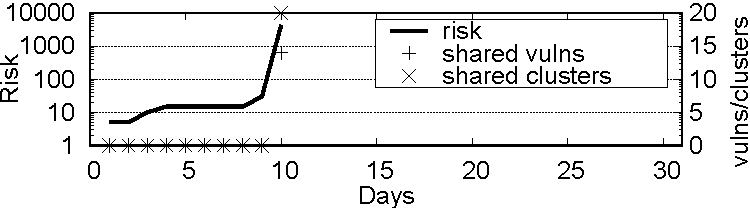
\includegraphics[width=0.5\columnwidth]{images/gnuplot/score/score_random_all.pdf}\label{fig:random_all}}
\hspace{0.5cm}
\subfloat[\system]{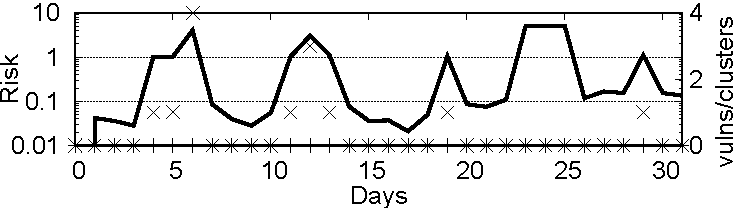
\includegraphics[width=0.5\columnwidth]{images/gnuplot/score/score_final_all.pdf}\label{fig:intel_all}}
\caption{Execution phase for Random and \system OS configuration strategies (log scale).}
\label{fig:run_all}
\end{figure*}

\textbf{Results:} As shown in Figure~\ref{fig:random_all}, \emph{Random} survives only for $10$ days. 
The number of shared clusters and vulnerabilities remains small for the first days. 
Then, there is a replica replacement that adds to the configuration an OS that has common vulnerabilities with the others. 
%Thus, enabling an adversary to compromise enough replicas in the system.

\system survives until the end of the experiment, as the risk is continually managed to keep the system safe. Figure~\ref{fig:intel_all} shows that shared clusters sometimes increase, at the same pace as the risk.
But then, the next reconfigurations are carried out with the goal of decreasing the risk. 
Notice that the risk value is always under $1$ for \system, and in the \emph{Random} is mostly above $10$.


\subsection{Diversity vs Attacks}

\begin{table}[t]
\begin{center}
{%\small%
\footnotesize
\begin{tabular}{ | p{0.96\columnwidth} | }\hline

\textbf{Samba:} 
\emph{On February 2, 2017, security researchers published details about a zero-day vulnerability in Server Message Block (SMB) of Windows, affecting several versions such as 8.1, 10, Server 2012 R2, and Server 2016. 
Could cause a \gls{dos} condition when a client accesses a malicious SMB.}\\
\textbf{CVES:} 
CVE-2017-0016
\\ \hline

\textbf{Wanna Cry:} 
\emph{On Friday, May 12, 2017, the world was alarmed to discover a widespread ransomware attack that hit organizations in more than 100 countries. Based on a vulnerability in Windows' SMB protocol (nicknamed EternalBlue), discovered by the NSA and leaked by Shadow Brokers.} \\
\textbf{CVES:} 
CVE-2017-0143, CVE-2017-0144, CVE-2017-0145, CVE-2017-0146, CVE-2017-0147, CVE-2017-0148 \\ \hline

\textbf{PowerShell:} 
\emph{Security feature bypass vulnerabilities in Device Guard that could allow an attacker to inject malicious code into a Windows PowerShell session.} \\
\textbf{CVES:}
CVE-2017-0219, CVE-2017-0173, CVE-2017-0215, CVE-2017-0216, CVE-2017-0218\\ \hline

\textbf{Stackclash:} 
\emph{In its 2017 malware forecast, SophosLabs warned that attackers would increasingly target Linux. The flaw, discovered by researchers at Qualys, is in the memory management of several operating systems and affects Linux, OpenBSD, NetBSD, FreeBSD and Solaris.}\\
\textbf{CVES:}
CVE-2017-1000365, CVE-2017-1000366, CVE-2017-1000367, CVE-2017-1000369, CVE-2017-1000370, CVE-2017-1000370, CVE-2017-1000371, CVE-2017-1000372, CVE-2017-1000373, CVE-2017-1000374, CVE-2017-1000375, CVE-2017-1000376, CVE-2017-1000379, CVE-2017-1083, CVE-2017-1084, CVE-2017-3629, CVE-2017-3630, CVE-2017-3631\\ \hline

\end{tabular}
}
\caption{Notable attacks during 2017.}
\label{tab:special_vulns}
\end{center}
\end{table}

This experiment evaluates the strategies when facing notable attacks/vulnerabilities that appeared in $2017$. 
Each attack potentially exploits several flaws, some of which affecting different \glspl{os}. 
The attacks were selected by searching the security news sites for high impact problems, most of them related to more than one CVE. 
As some of the \glspl{cve} include applications, we added more vulnerabilities to the database for this purpose.
Table~\ref{tab:special_vulns} lists the attacks and related \glspl{cve}: Samba,\footnote{https://www.secureworks.com/blog/attacking-windows-smb-zero-day-vulnerability} WannaCry,\footnote{https://securityintelligence.com/wannacry-ransomware-spreads-across-the-globe-makes-organizations-wanna-cry-about-microsoft-vulnerability/} Powershell,\footnote{http://blog.talosintelligence.com/2017/06/ms-tuesday.html} and Stackclash.\footnote{https://nakedsecurity.sophos.com/2017/06/20/stack-clash-linux-vulnerability-you-need-to-patch-now/}


Since some of these attacks might have been prepared months before the vulnerabilities are publicly disclosed, we augmented the execution phase to the full six months. 
As before, the strategies are analyzed over $5000$ runs.


\begin{figure}[t]
\begin{center}
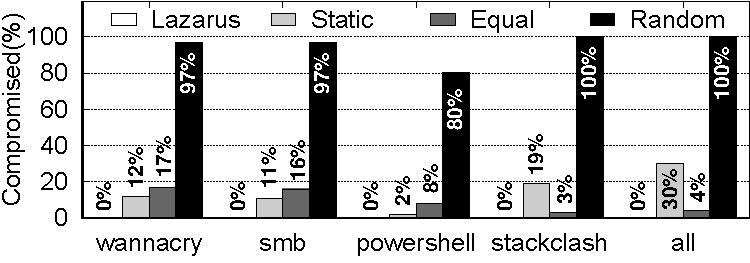
\includegraphics[width=\columnwidth]{images/gnuplot/special_vulns/execution-special.pdf}
\caption{Compromised runs with notable attacks.}
\label{fig:special_vulns}
\end{center}
\end{figure}

\textbf{Results:}
Figure~\ref{fig:special_vulns} shows the percentage of compromised runs for each attack and all attacks put together.
\system is clearly the best at handling the various scenarios, with no compromised executions.
\emph{Random} is the worse, as it does not use any criteria to select the OSes. 
Both \emph{Equal} and \emph{Static} may perform not so bad as they are static, i.e., the \glspl{os} selected by random chance might end up not being exploitable until the end of the run.

\section{Final Remarks}
\label{sec:finalremarkslazarus}

\system addresses the long-standing open problem of evaluating, selecting, and managing the diversity of a \gls{bft} system to make it resilient to malicious adversaries.
Our work focuses on two fundamental issues: how to select the best replicas to run together given the current threat landscape, and what is the performance overhead of running a diverse \gls{bft} system in practice.

